\section*{Neural Networks}
There are several categories of statistical algorithms for data analysis within machine learning.
Amongst them are neural networks, which have for the last decade exponentially been used
within industry and academia for a number of usecases. From image analysis to weather prediction,
these models are used extensively. \par
Neural networks, or feed forward neural networks (FFNN), are based on a few principles.
First, the data is feeded forward through the network. The end output is evaluated in some fashion, 
and corrections are then back propagated through the network, updating the weights and biases. 
This "training" is done until a sufficient threshold is met. A general layout of a neural network is displayed in
figure \ref{fig:nndiagram}.

\begin{figure}
    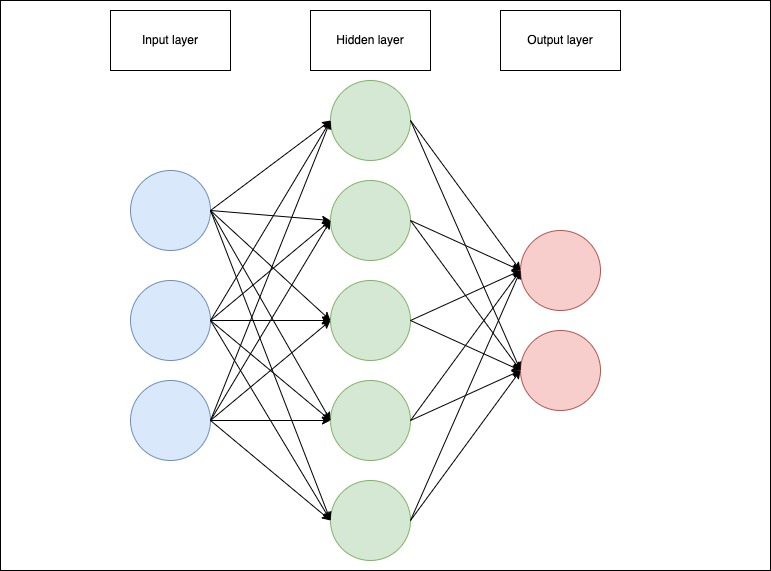
\includegraphics[width=\linewidth]{Figures/Machinelearning/nn_diagram.jpeg}
    \caption{Simple neural network diagram drawm using Draw.io. Here the blue dots are the input layer, the green dots are a hidden layer, 
    and the red dots are the output layer. The arrows shows the connections between each node. }
    \label{fig:nndiagram}
\end{figure}

The input layer has the same shape of the dataset one uses to train or predict on, with one node for each feature in the dataset.
The next layer is the hidden layers. For a given network, the amount of hidden layers can be tuned, as well as the number of 
nodes per layer. Finally, the last hidden layer is connected to the ouput layer, which is determined by the aim of the problem. 
In the case of figure \ref{fig:nndiagram}, this neural network would represent a binary classification problem, in other words, two categories. 
The nodes in the network interacts through so called weights $w$ and biases $b$. These are known as tunable parameters, 
which needs to be trained on the dataset before any prediction can be made. 

\subsection*{Gradient descent}
Let us now consider a general n-dimansional problem, with parameters $\boldsymbol{\theta} = \{\theta_1, \theta_2, ..., \theta_n\}$. We want the set of $\boldsymbol{\theta}$
such that we minimize a costfunction with respect to the data and target. One way to solve this problem is using ordinary least squares. For this approach, 
the optimal paramters $\boldsymbol{\theta_{opt}}$ are derived from minimizing the cost function, as shown here:
\begin{equation*}
    \boldsymbol{\theta_{opt}} = (\boldsymbol{X}^T\boldsymbol{X})^{-1}\boldsymbol{X}^T\boldsymbol{t},
\end{equation*}
where $\boldsymbol{X}$ is the design matrix containing the data, and $\boldsymbol{t}$ is the target vector. This however leads to a problem. Suppose the design matrix is sufficiently large,
then the matrix inversion will get computaitonally expensive, or it might not even exist for a given $\boldsymbol{X}$. Thus, an alternative approch is to iteratively approximate the the ideal 
parameters. \par 
Suppose we we have a cost function $C(\boldsymbol{\theta})$ for a given problem. We can approximate the minimum of the cost function by calculating
the gradient $\nabla_{\theta}C$ with respect to $\boldsymbol{\theta}$. The negative of this gradient indicates the direction for the minimum of $C$ when evaluating 
it in a specific point $\boldsymbol{\theta}_i$ in the parameter space \cite{FYSSTK}. This is formulized as follows 
\begin{equation}
    \boldsymbol{\theta}_{i+1} = \boldsymbol{\theta}_i - \eta\nabla_{\theta}C(\boldsymbol{\theta}_i),
\end{equation}
where $\eta$ is a step size, also called the learning rate. The choice of $\eta$ is not a trivial case. It is one of severel 
hyperparameters\footnote{Give reference to hyperparameters}
that can be altered, and that highly depend on the given problem. with regards to the learning rate, there are only three situations to consider, shown in figure \ref{fig:lr_choice}.
\begin{figure}
    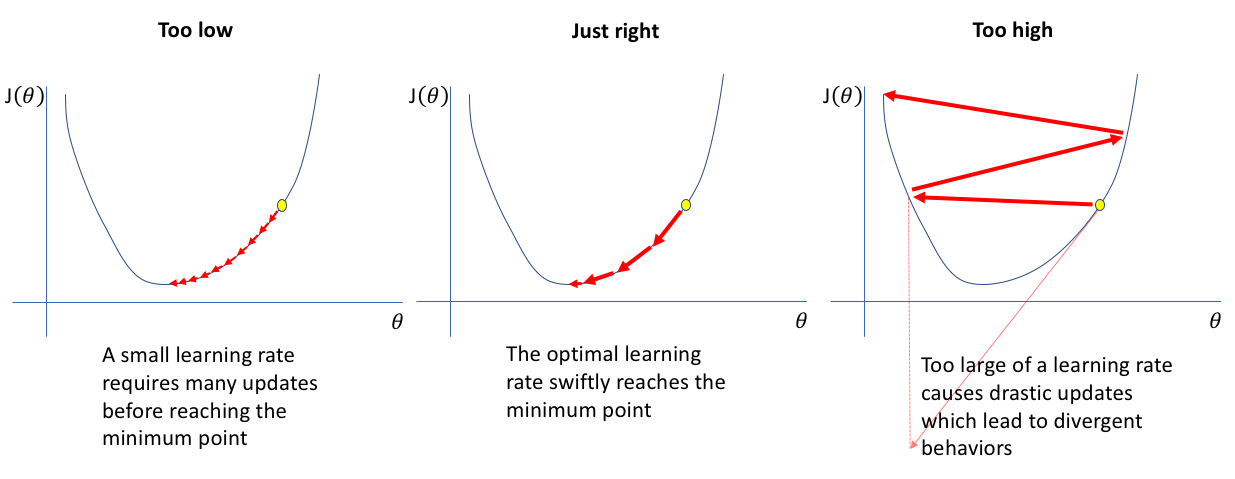
\includegraphics[width=\linewidth]{Figures/Machinelearning/lr_choice.png}
    \caption{Figures showing different choice of learning rate for a given costfunction, with respect to the tunable parameters. 
    Source: \href{https://www.jeremyjordan.me/content/images/2018/02/Screen-Shot-2018-02-24-at-11.47.09-AM.png}{Jeremy Jordan}, accessed 03.10.22.}
    \label{fig:lr_choice}
\end{figure}

Figure \ref{fig:lr_choice} visualizes the relation between the learning rate and the cost function. In the left most figure we note that the learning rate is too small. 
This leads to many iterations before you reach a minimum. In the right most figure we note that the learning rate is too high, and the result is that we get divergent behavior. 
Thus the goal is to find the optimal learning rate, shown in the middle figure. \par 
A modified and prefered version of gradient descent is the so called stochastic gradient descent. Regular gradient descent can, for large datasets be quite slow, and is prone to 
getting stuck in local minima. To circumvent this issue, mini batches are introduced. 






\subsection*{Backpropagation}

\subsection*{Feed forwarding}